
\documentclass[12pt, a4paper]{article}
\usepackage[utf8]{inputenc}
\usepackage[T1]{fontenc}
\usepackage{pgfplots}
\usepackage{tikz}
\usepackage{amssymb}
\usepackage{amsmath}
\usepackage{amsfonts}
\usepackage{graphicx}

\pgfplotsset{compat=1.18, width=10cm}

\begin{document}
\tableofcontents
\newpage
\section{Precalculus}
\subsection{Algebra}
\subsection{Trigonometry}
\section{Calculus}
\section{Linear Algebra}
\subsection{Wektor}
Wektor to uporządkowana para liczb. Jeśli wektor ma początek to jest to, wektor
zaczepiony który jest oznaczany symbolem $\overrightarrow{AB}$. Jeżeli dane są punkty
$A = (x_1,y_1)$ oraz $B = (x_2,y_2)$,
to współrzędne wektora $\overrightarrow{AB}$ określa wzór: $$\overrightarrow{AB} = [x_2-x_1,y_2-y_1]$$
Jeśli natomiast wektor nie ma początku to jest to wektor swobodny który
jest oznaczany symbolem $\overrightarrow{v}, \overrightarrow{u}, \overrightarrow{w}$.
$$\overrightarrow{u} = \overrightarrow{w} \Longleftrightarrow u_x = w_x \wedge u_y = w_y$$
Na rysunku poniżej został przedstawiony wygląd wektora $[3,2]$ i $[-2,4]$ w układzie współrzędnych:

\begin{center}
\begin{tikzpicture}
\begin{axis}[xmin=-4.5,xmax=4.5,ymin=-2.5,ymax=4.5,axis lines=middle,
            xtick={-4,-3,...,4},ytick={-4,-3,...,4}, xlabel=$x$, ylabel=$y$,
            ]
  \addplot[domain=0:4, samples=250, ultra thick,blue, ->] coordinates {
    (0,0)
    (3,2)
  }
  node[pos=1.0, above left, blue]{$[3,2]$};
  \addplot[domain=0:4, samples=250,dashed] coordinates {
    (0,2)
    (3,2)
    (3,0)
  };

  \addplot[domain=0:4, samples=250, ultra thick,red, ->] coordinates {
    (0,0)
    (-2,4)
  }
  node[pos=1.0, below left, red]{$[-2,4]$};
  \addplot[domain=0:4, samples=250,dashed] coordinates {
    (0,4)
    (-2,4)
    (-2,0)
  };

\end{axis}
\end{tikzpicture}
\end{center}
Długość wektora $\overrightarrow{w}$ oraz $\overrightarrow{AB}$ można zapisać następująco:
$$|\overrightarrow{w}| = \sqrt{w^2_x + w^2_y}$$
$$|\overrightarrow{AB}| = \sqrt{\left(x_2 - x_1\right)^2 \left(y_2 - y_1\right)^2}$$
gdzie:
\begin{itemize}
  \item $A(x_1,y_1)$ i $B(x_2,y_2)$ to długości wektora $\overrightarrow{AB}$
\end{itemize}
\vspace{1em}
Sumą, różnicą, iloczynem $\overrightarrow{u} = [u_x,u_y]$ i $\overrightarrow{w} = [w_x,w_y]$, wyraża się wzorem:
$$\overrightarrow{u} + \overrightarrow{w} = [u_x + w_x, u_y + w_y]$$
\begin{center}
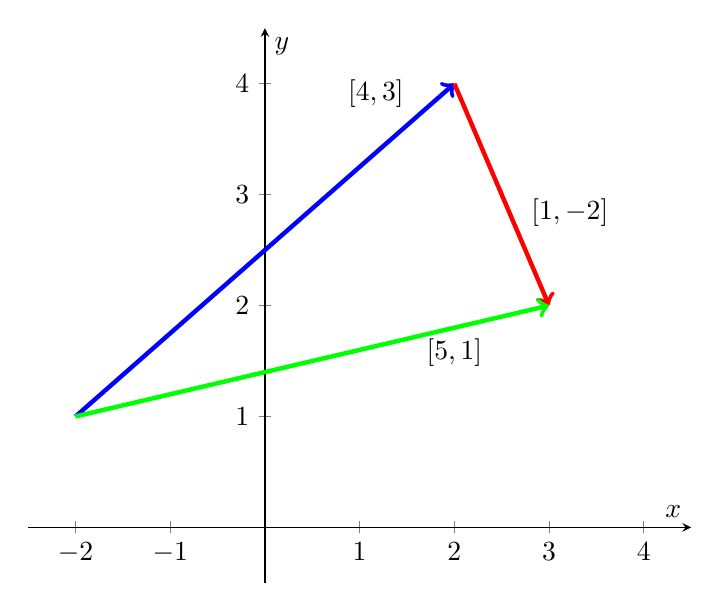
\begin{tikzpicture}
\begin{axis}[xmin=-2.5,xmax=4.5,ymin=-0.5,ymax=4.5,axis lines=middle,
            xtick={-4,-3,...,4},ytick={-4,-3,...,4}, xlabel=$x$, ylabel=$y$,
            ]
  \addplot[domain=0:4, samples=250, ultra thick,blue, ->] coordinates {
    (-2,1)
    (2,4)
  }
  node[pos=1.0, above = -0.125cm, left = 0.50cm, black]{$[4,3]$};
  \addplot[domain=0:4, samples=250, ultra thick,red, ->] coordinates {
    (2,4)
    (3,2)
  }
  node[pos=0.9, above = 0.9cm, right = -0.25cm, black]{$[1,-2]$};
  \addplot[domain=0:4, samples=250, ultra thick,green, ->] coordinates {
    (-2,1)
    (3,2)
  }
  node[pos=0.8, below, black]{$[5,1]$};
\end{axis}
\end{tikzpicture}
\end{center}
$$\overrightarrow{u} - \overrightarrow{w} = [u_x - w_x, u_y - w_y]$$

\begin{center}
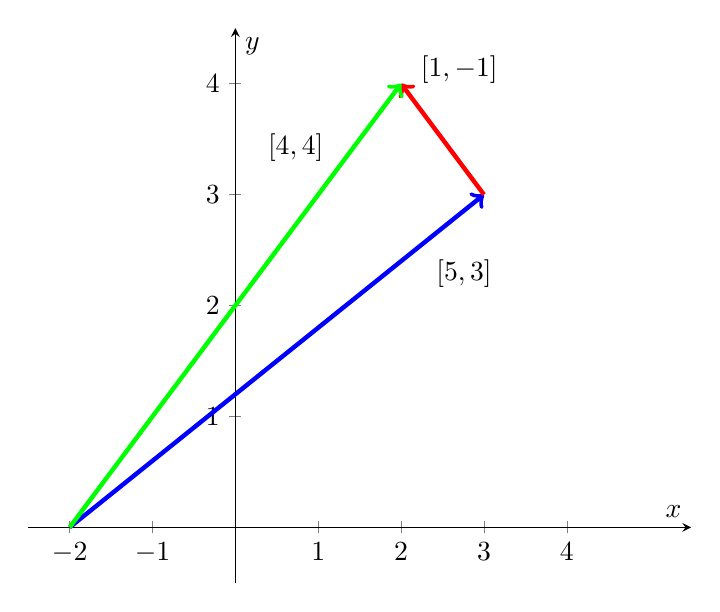
\begin{tikzpicture}
\begin{axis}[xmin=-2.5,xmax=5.5,ymin=-0.5,ymax=4.5,axis lines=middle,
            xtick={-4,-3,...,4},ytick={-4,-3,...,4}, xlabel=$x$, ylabel=$y$,
            ]
  \addplot[domain=0:4, samples=250, ultra thick,blue, ->] coordinates {
    (-2,0)
    (3,3)
  }
  node[pos=1.0, below = 1cm, right = -0.75cm, black]{$[5,3]$};

  \addplot[domain=0:4, samples=250, ultra thick,red, ->] coordinates {
    (3,3)
    (2,4)
  }
  node[pos=0.9, above right, black]{$[1,-1]$};

  \addplot[domain=0:4, samples=250, ultra thick,green, ->] coordinates {
    (-2,0)
    (2,4)
  }
  node[pos=0.8, above left, black]{$[4,4]$};
\end{axis}
\end{tikzpicture}
\end{center}
$$ a \cdot \overrightarrow{w} = [a \cdot w_x, a \cdot w_y], \quad \text{gdzie } a \in \mathbb{R}$$
\begin{center}
\begin{tikzpicture}
\begin{axis}[xmin=-3.5,xmax=2.5,ymin=-3.5,ymax=2.5,axis lines=middle,
            xtick={-4,-3,...,4},ytick={-4,-3,...,4}, xlabel=$x$, ylabel=$y$,
            ]
  \addplot[domain=0:4, samples=250, ultra thick,blue, ->] coordinates {
    (0,0)
    (1,1)
  }
  node[pos=1.0, above right, black]{$[5,3]$};

  \addplot[domain=0:4, samples=250, ultra thick,red, ->] coordinates {
    (0,0)
    (-2,-2)
  }
  node[pos=0.9, below left = 0.25cm, black]{$[-2,-1]$};
\end{axis}
\end{tikzpicture}
\end{center}
Wektory $\overrightarrow{u} = [u_x, u_y]$ i $\overrightarrow{w} = [w_x, w_y]$, są przeciwne wtedy,
gdy suma wektorów $\overrightarrow{u}$ i $\overrightarrow{w}$ jest wektorem zerowym, czyli:
$$\overrightarrow{u} = -\overrightarrow{w} \Longleftrightarrow u_x + w_x = 0 \wedge u_y + w_y = 0$$
\end{document}
